\documentclass[9pt,a4paper,twoside]{tau}
\usepackage[english]{babel}
\usepackage{tauenvs}

%----------------------------------------------------------
% TITLE
%----------------------------------------------------------

\title{Investigative Report of Franklin Resources Inc. [stock:BEN]from April 2022 to April 2024}

%----------------------------------------------------------
% AUTHORS, AFFILIATIONS AND PROFESSOR
%----------------------------------------------------------

\author[a,1]{Bucsa, Justin}

%----------------------------------------------------------

\affil[a]{Stealth}
\professor{}

%----------------------------------------------------------
% FOOTER INFORMATION
%----------------------------------------------------------

\institution{Stealth}
\ftitle{}
\date{April 19, 2024}
\etal{Bucsa}
\course{}

%----------------------------------------------------------
% ABSTRACT
%----------------------------------------------------------

\begin{abstract}    
    This report provides a comprehensive analysis of Franklin Resources Inc. (BEN) as a potential investment opportunity. It examines the company's performance over a two-year period (April 2022 - April 2024), encompassing historical background, strategic goals, and major shareholder structure. We will delve into market data to understand BEN's price movements and analyze key events that transpired within the past year (April 2023 - April 2024) to assess their impact. Finally, the report culminates in a holistic evaluation of Franklin Resources Inc.'s investment potential.

\end{abstract}

%----------------------------------------------------------
% \keywords{}
%----------------------------------------------------------

\begin{document}
		
	\maketitle
	\thispagestyle{firststyle}
	\tauabstract
	\tableofcontents

%----------------------------------------------------------

\section{Introduction}

    \taustart{F}ranklin Resources Inc. [NYSE:BEN], is one of the world's largest investment managers, is better known as Franklin Templeton. It currectly over sees \$1.6 trillion in total assets under management, over 1400 investment professionals in 25 counties and over 9000 employees globally. In this report will first discuss

\section{History}
    Franklin Resources boasts a rich history dating back to 1947, when it began operations in the investment management field. The company initially focused on mutual funds, offering both fixed income and equity options (growth and value-oriented). Through strategic acquisitions, Franklin has continuously expanded its reach and expertise. Notable additions include:

    - 1992: Templeton, a global investment firm, bringing international investment capabilities.
    
    - 1996: Franklin Mutual Series, further solidifying its mutual fund portfolio.

    - 2000 \& 2001: Acquisitions like Franklin Bissett Canadian and Fiduciary Trust International broadened their offerings to include Canadian investment management and trust services.
    
    - 2019-2022: A period of significant expansion, with acquisitions like Benefit Street Partners (alternative credit), Athena Capital Advisors (wealth management), Legg Mason (global investments), O’Shaughnessy Asset Management (quantitative assets), Lexington Partners (alternative investments), and Alcentra (alternative credit).
    
    This strategy of growth through acquisitions has transformed Franklin Resources into a leading global investment management firm with a diverse range of offerings to meet evolving investor needs.
    
\section{Events}

    \subsection{May 2023 - Acquisition of Putnam Investments Announced}
	
        Franklin Resources Inc. announced a significant acquisition in May 2023, entering into a definitive agreement to acquire Putnam Investments from Great-West Lifeco. Inc. (Great-West), a member of the prominent Power Corporation group. This strategic move strengthens Franklin Templeton's position in the asset management industry. Great-West and Power Corporation are leaders in global insurance, retirement, wealth management, and asset management, aligning well with Franklin Templeton's existing strengths. The acquisition was expected to close in the first quarter of fiscal year 2024, subject to customary closing conditions.

    \subsection{January 2024 - Acquisition of Putnam Investments Completed}
	
        Franklin Resources Inc. successfully completed the acquisition of Putnam Investments, expanding its global footprint and AUM (Assets Under Management). This strategic move solidified Franklin Resources' position as a leading investment management firm.
    
    \subsection{Insider Sales}
        Below is a list of Insider stock sales from members of Franklin Resources Inc. exectives and board of directors from 2022-04-20 to 2024-04-20.
    
    
            \begin{figure}[H]
                \centering
                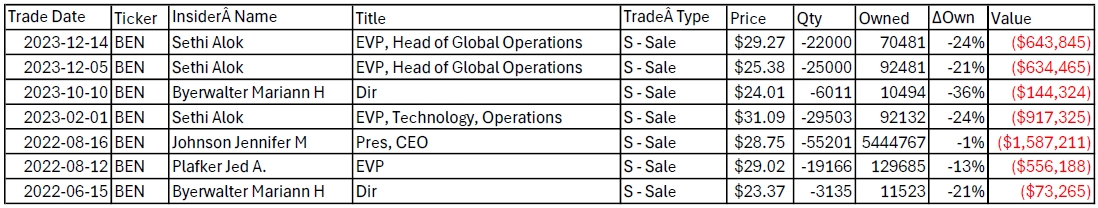
\includegraphics[width=0.95\columnwidth]{images/InsiderTrades.jpg}
                \caption{This is a table of Insider Trades from 2022-04-20 to 2024-04-20.}
                \label{fig:figure}
            \end{figure}

\section{Ownership Distribution}
    \subsection{Breakdown}
        Franklin Resources Inc. [NYSE:BEN] is divided into four categories of ownership: Insiders, Mutual Funds, Other Institional Investors, and Public Companies and Individual Investors. The pie chart below shows the distribution of ownership, were Insiders own the most at 40.88\% followed by Public Companies and Individual Investors at 25.85\%, Other Institional Investors at 19.77\% and finally Mutual Funds at 13.50\%.

            \begin{figure}[H]
                \centering
                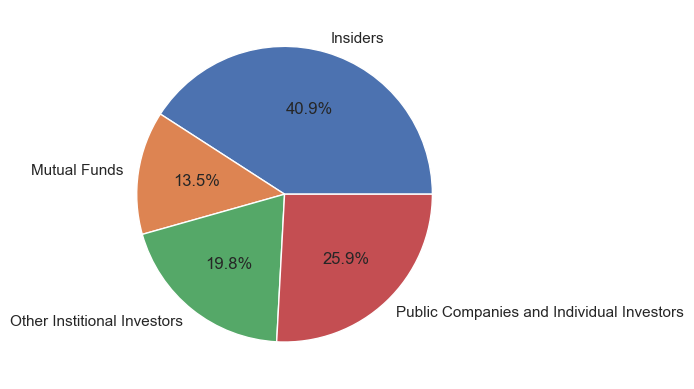
\includegraphics[width=0.85\columnwidth]{images/OwnershipPieChart.png}
                \caption{This chart represents how the shares of BEN are divided up as of 2024-04-20.}
                \label{fig:figure}
            \end{figure}

    \subsection{Concerns}
    
        Franklin Resources Inc. (NYSE: BEN) can be susceptible to immediate stock price swings. With a large portion of the ownership concentrated in insiders, public companies, and other institutional investors (holdings totaling 86.5\%) compared to mutual funds, the stock price could react more dramatically if these major investors decide to sell.  This concentration of ownership suggests that BEN might be a more stable choice for short-term investment strategies, but for long-term investors, the vulnerability to large investor sentiment should be a consideration

\section{Market Analysis}
    \subsection{Introduction to Market Analysis}
        This section will be focused on examining the Closing Price and Quarterly Revenue of Franklin Resources Inc. (NYSE: BEN) from 2022-04-20 to 2024-04-20. We will discuss possible impacts to each respectively and then compare both together.
    
    \subsection{Closing Price}
        Below is the Closing Cost of Franklin Resources Inc. (NYSE: BEN) per month from 2022-04-20 to 2024-04-20.
            \begin{figure}[H]
                \centering
                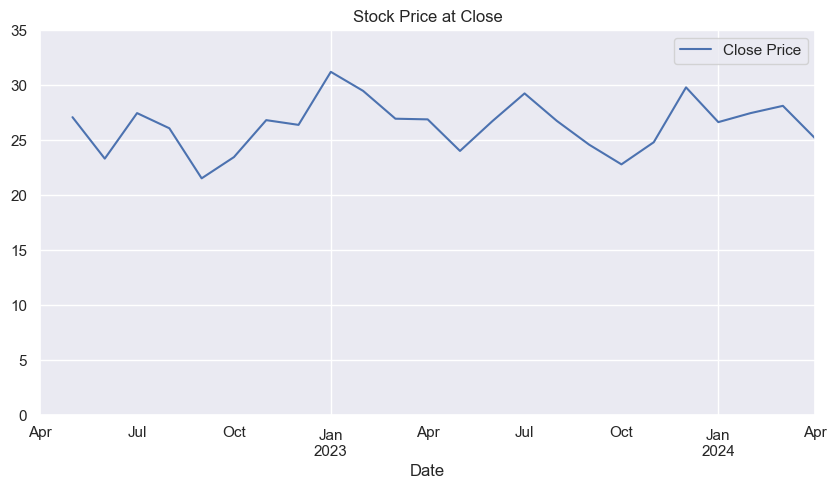
\includegraphics[width=0.85\columnwidth]{images/CloseDataSet1mo.png}
                \caption{This chart represents the Closing Stock Price per Month from 2022-04-20 to 2024-04-20.}
                \label{fig:figure}
            \end{figure}
        The price appears to be in a flux of plus or minus \$5.00 every quarter, a rate of change near 16.67\% of the stock value. In fact, if we look at the daily trades, we can see the jumps more clearly occur at a quartly period. 
            \begin{figure}[H]
                \centering
                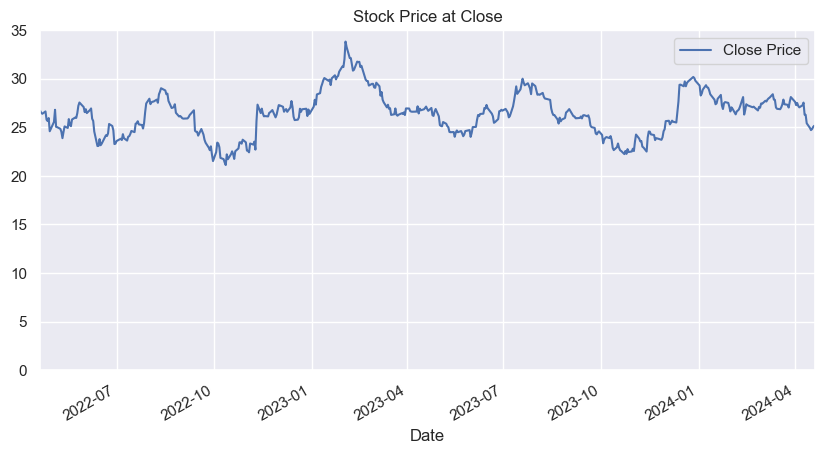
\includegraphics[width=0.85\columnwidth]{images/CloseDataSet1d.png}
                \caption{This chart represents the Closing Stock Price per Day from 2022-04-20 to 2024-04-20.}
                \label{fig:figure}
            \end{figure}
        If we compare the two charts together, we can see the month average trails the daily report due to this large jumps in the Closing Price.
            \begin{figure}[H]
                \centering
                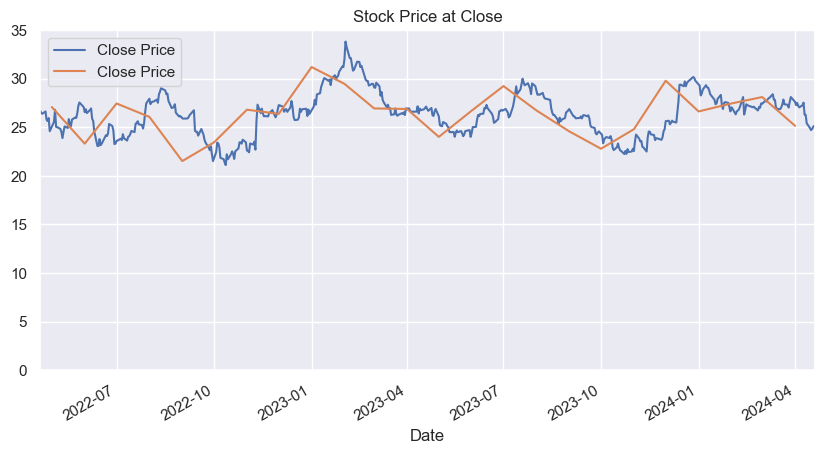
\includegraphics[width=0.85\columnwidth]{images/CloseDataSet1dvs1mo.png}
                \caption{This chart represents the Closing Stock Price per Day vs. Closing Stock Price per Month from 2022-04-20 to 2024-04-20.}
                \label{fig:figure}
            \end{figure}
        This leads us to comclude there is a market force acting on the start that makes it visiable for a daily trading over monthly trading. 

        Let us continue into the Quarterly Revenue reports.

    \subsubsection{Quarterly Revenue}
        Since Franklin Resources Inc. [NYSE:BEN] does have over \$1.6 trillion in asset under managerment, we can see their earnings report show a profit of sometimes breaking \$200 billion in recently quarter. Below is a chart show the recent Quarter Revenue from 2022-04-20 to 2024-04-20.
            \begin{figure}[H]
                \centering
                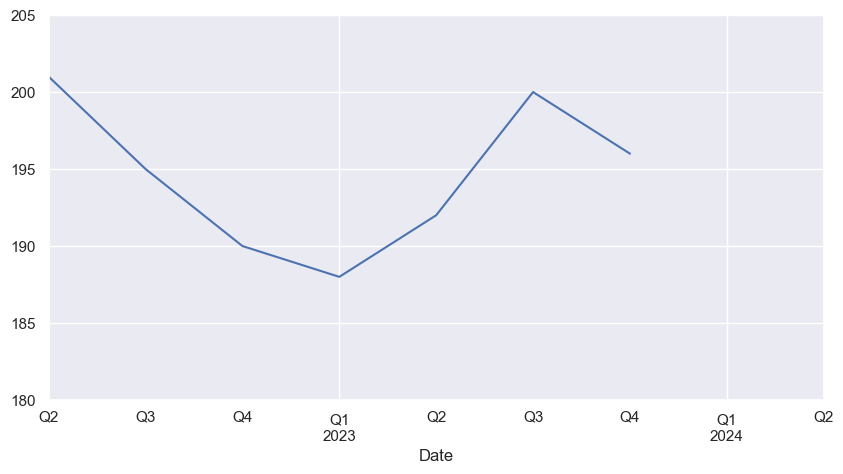
\includegraphics[width=0.85\columnwidth]{images/EarningByQt.png}
                \caption{This chart represents the report earning in Billions over the quarters from 2022-04-20 to 2024-04-20.}
                \label{fig:figure}
            \end{figure}
        It appears that the revenue of Franklin Resources Inc. [NYSE:BEN] does fluxate plus or minus \$5 billion, coming to a rate of change near 2.5\%.  That means the stock value has a rate of change nearly 666.8\% higher than the rate of change of the revenue. 
            
    \subsubsection{Closing Price vs. Quarterly Revenue}   
        Let us now just simple compare the Closing Price of the stock to the Quarterly Revenue. We will do this by laying the Quarterly Revenue chart onto the Closing Price chart. Note that Y-axis for the right is the value of the stock and the Y-axis to the left is the Gross Revenue value in billions. The x-axis is the same for both.  
            \begin{figure}[H]
                \centering
                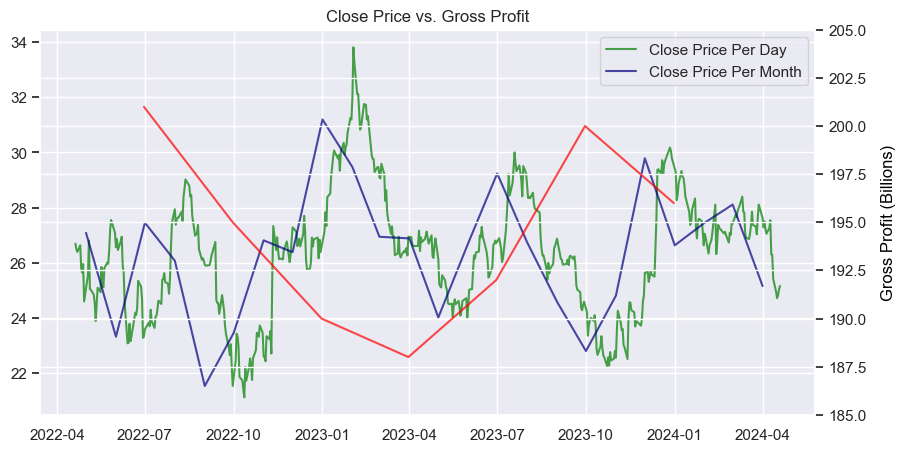
\includegraphics[width=0.85\columnwidth]{images/CloseDataVsProfit.png}
                \caption{This chart compares the monthly and daily closing price against the reported quartly earning price (in red) 2022-04-20 to 2024-04-20.}
                \label{fig:figure}
            \end{figure}
        Now we can see that change in the stock value is inversely related to the reported revenue. What is causing this?

        Well in May 2023, the stock was rising due to the new of the merger, but the cost of the merger was impacting the profit at that time. Thus when the following revenue reports came out, investors paniced and the stock dropped. But after the merger, the company was becoming more profitable due to the completion of the merger, but investors still had not return to the stock. 
        It was not it the following earning report, did the investor come back. 
        As of the most recently quartly report, we see that the profit not being continuously positive, is having another negative impact on the stock value of Franklin Resources Inc. [NYSE:BEN]. This means, even one quartly report that is not exceed \$200 billion in revenue, will have a drastic impact on the stock price. 



\section{Conclusion}
    \subsubsection{Short Term}
       Franklin Resources Inc. [NYSE:BEN] is an active stock that has a ideal flux or rate of movement for day trading. Even through it does appear to be moving in a downward direction, it is still based upon a large profit companies. Thus, if the stock drops 5\%-10\% in an day, there is a good chance it will recover in a positive direction the following day or even within the same day of trading.

    \subsubsection{LongTerm}
        Not the most ideal for long term investments. Franklin Resources Inc. [NYSE:BEN] appears to rely heavily on acquisitions at the current time to remain profitable in the long term. Which is great, if the short-term investor did not effect value as dramatically as they do. Just looking at the most recent dating for the late two years, an investor barely broke even due to fluxation caused by the day trading community. 
        For that, a long term investment may over see a return of 2\% to 5\% beyond a 2 year time frame. For that reason, no long term investor should invest in Franklin Resources Inc. [NYSE:BEN] when other S\&P stocks have proven to be much more reliable over the long term. 
%----------------------------------------------------------

\addcontentsline{toc}{section}{References}
\printbibliography


%----------------------------------------------------------

\begin{center}

	\textit{Contact:} \\

	\faEnvelope[regular]\ justin.bucsa@gmail.com \\

\end{center}

%----------------------------------------------------------

\end{document}